% this file is called up by thesis.tex
% content in this file will be fed into the main document

\chapter{Related Work} % top level followed by section, subsection


% ----------------------- paths to graphics ------------------------

% change according to folder and file names
\ifpdf
    \graphicspath{{7/figures/PNG/}{7/figures/PDF/}{7/figures/}}
\else
    \graphicspath{{7/figures/EPS/}{7/figures/}}
\fi


% ----------------------- contents from here ------------------------
% 

\section{Support Technologies}

Several developments across different fields have been essential for the
goals we envision for CSx. In this section we go to the most prominent of 
these developments. However, only developments not directly related to CSxs are
covered as the next section covers these CSx developments in detail.

These developments are three fold. Firstly, the development of host-managed
storage interfaces with first \textit{Open-Channel SSD} (OCSSD)
\cite{Bjrling2017LightNVMTL} and later NVMe ZNS. Secondly, filesystem
improvements with F2FS \cite{Lee2015F2FSAN} using an optimized layout for flash
storage devices. Lastly, a heterogenous compute ISA, namely eBPF
\cite{ebpf_cs_2021, kourtis2020safe, bpf-uapi}.

OCSSD exposes the flash layout through an end user API \cite{liblightnvm}.
Effectively, this moved the FTL with wear-leveling and gargabe collection
functionality to the host. However, the intricate details of this flash layout
made the API hard to use for users as well as implement for SSD vendors. In
addition, vendors might fear that exposing all these details could leak trade
secrets. A more succesful alternative to OCSSD is NVMe ZNS which is now a
ratified extension to the NVMe specification \cite{nvme-zns}. In NVMe ZNS the
flash layout is exposed in zones. Subsequently, all sectors in a zone must be
written in a sequentially incremented fashion as well as the entire zone must
be erased as a whole. Finally, ZNS devices can impose limits on the maximum
amount of zones that can be opened at any given time. This zoned layout is
visually compared to a conventional flash SSD in figure \ref{figure:znslayout}.

\begin{figure}[H]
    \centering
	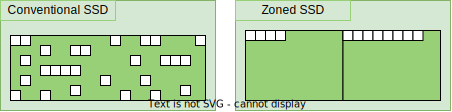
\includegraphics[width=0.8\textwidth]{resources/images/zns-vs-conventional-layout.pdf}
	\caption{Comparison of conventional and ZNS SSD data layouts}
    \label{figure:znslayout}
\end{figure}

This new ZNS technology has already been used in promising research avenues such
as an optimized garbage collection scheme \cite{254268}. In addition, we see
a more general performance evaluations \cite{10.1145/3458336.3465300, 9188086}
demonstrating the advantages of ZNS. Lastly, we see proposals to extend the ZNS
interface to better support compaction in LFSs \cite{273709}.

% Transition sentence?

It is only recently that we have seen filesystems optimized for flash outside of
embedded applications. This new filesystem, F2FS \cite{Lee2015F2FSAN}, is
significantly more advanced than embedded filesystem like JFFS2 \cite{jffs2}.
With F2FS write-amplification is not only prevented by utilizing the sequential
write behavior of LFSs, in addition, it is prevented by tracking inode locations
in a separate NAT as oppossed to chaining inode location data together. This
flattened layout solves the wandering tree problem where a single location
updates causes a chain of updates to propagate. Other improvements include
separate logs for hot and cold data as well as garbage collection using a
\textit{Segment Info Table} (SIT) and \textit{Segment Summary Area} (SSA).
However, F2FS still has several limitations such as no wear-leveling and only
entirely invalidated zone garbage-collection. An overview of the F2FS data
layout is shown in figure \ref{figure:f2fslayout}.

\begin{figure}[H]
    \centering
	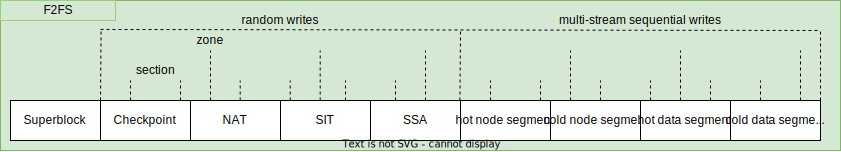
\includegraphics[width=1\textwidth]{resources/images/f2fs-layout.png}
	\caption{Overview of data layout on F2FS}
    \label{figure:f2fslayout}
\end{figure}

% Transition sentence?

eBPF is used in the Linux kernel extensively and is still seeing increasing use
cases. One of these recent new use cases is as heterogenous ISA \cite{bpf-uapi}.
The combination of the ease of virtualization together with the call instruction
enables to separate an API from its actual implementation. Even more, the
implementation is so separated from its implementation that it does not have to
be linked at compile time or even be present on the host system. Previous works
have already explained why eBPF is such a good fit for computational storage in
detail \cite{ebpf_cs_2021}. Lastly, the capabilities of eBPF have already been
demonstrated in the case of disaggregated storage \cite{kourtis2020safe}.

\section{Computational Storage Devices}

While OpenCSD is unique it is by no means the first CSx prototype as there
has been over a decade of research in this field \cite{lukken2021past}. In this
decade we have seen a large variety of approaches, problem spaces, hardware
platforms and software APIs. There is significant progression in this field, 
however, several important challenges are still open research
questions \cite{barbalacecomputational}.

In this section we introduce characteristics of CSx prototypes, the most
prominent open research questions, provide an overview of notable works,
describe the progression of the field and describe fundamentally missing
features that hinder adoption and widespread use of CSxs.

% Introduce early working prototypes

% Demonstrate different hardware platforms, embedded CPU, vs FPGA.

% List of BPF using storage literature (Blockndp:, Extos: Data-centric
%extensible os, Ex-tension framework for file systems in user space, 
%  Safe and efficient remote application code execu-tion on disaggregated NVM,
% BPF for storage: an exokernel-inspired approach )

% Introduce previous ZCSD table but extended

\subsection{CSx characterstics}

There are four types of characteristics that set CSxs apart. First there is
the end user \textit{programming model}, the model of programming developers
have to use in order to interact with CSx. Second, there is the execution
environment, the level of software abstraction the end user programs are run on
(on the device). Third, is the \textit{degree of programmability}, the amount of
programming control offered to the end user. Lastly, there is the interface used
to connect the device to the host.

With end user programming models there are, in no particular order,
\textit{Dataflow (MapReduce, DAG)}, \textit{Client / Server
(RPC \footnotemark[1], HTTP \footnotemark[2])}, \textit{Shared memory} and
\textit{Declarative (Regex, MySQL)}. Although simple categories, the correct
attribution of these categories can become quite complicated due to nuances. For
instance, if an end user needs to link to a new shared library to call methods
with MySQL queries as argument it becomes unclear what the programming model
should be. In this work we argue \textit{Shared memory} as the library that
needs to be linked is introduced in the work.

\footnotetext[1]{\textit{Remote Procedure Call} (RPC)}

\footnotetext[2]{\textit{HyperText Transfer Protocol} (HTTP)}

In \textit{Computational Storage Execution Environments} (CSEE) we effectively
observe seven distinct levels of abstraction. These range from
\textit{Register-Transfer Level} (RTL) design such as using languages like
Verilog or VHDL to virtual machines. The compiled output of RTL designs is known
as a bitstream and typically programmed into an FPGA at runtime. The distinct
levels are listed below.

\begin{enumerate}
    \item Bistream; bitstream programmed directly unto FPGA.
    \item Embedded; single program, single memory space, no OS just 'real mode'.
    \item Accelerators; OpenCL, Vulkan.
    \item Real-Time operating system;
    \item Operating System;
    \item Container;
    \item Virtual Machine;
\end{enumerate}

We see a similarly large range in different \textit{degrees of programmability}
from no end user programmability at all such as with transparent operations to
arbitrary code execution. The six distinct levels are shown below. It
should be noted, howerver, that the first two levels can be regarded as no or a
lack of end user programmability.

\begin{enumerate}
    \item Transparent operations, (de)compression (Playstation 5 I/O Controller)
    \item Fixed functions, unchangeable, workload specific \cite{2013-fast-active-flash}
    \item Fixed function dataflow programming \cite{Wickremesinghe02distributedcomputing}
    \item Query offloading, SQL\footnotemark[3], NoSql, Regex \cite{10.14778/2994509.2994512}
    \item Event driven (hooks) user-programmable functions \cite{10.1145/3429357.3430519}
    \item Arbitrary code execution, VHDL, eBPF, TCL \cite{10.1145/605432.605425, kourtis2020safe}
\end{enumerate}

\footnotetext[3]{\textit{Structured Query Language} (SQL)}

It is important to illustrate that the \textit{degree of programmability} is
fundamentally different from the end user \textit{programming model} as one
denotes how programs are submitted and run on the device while the other denotes
what model an end user must use to develop for the CSx respectively.

\subsection{Past CSx Works}

Using these characteristics of CSxs allows to make a qualitative comparison of
different works from the past decade. By arranging all these works in
publication order as shown in table \ref{table:csxoverview} we can start to
obeserve developments in the field. We describe three different types of
observations being general observations, observations relating to changes over
time and finally observations on specific works.

Firstly, we can observe that the amount of works with a limited \textit{degree
of programmability} is small, consisting of just \textit{Active Flash
\cite{active-flash-piller, 2013-fast-active-flash},
Caribou \cite{10.14778/3137628.3137632}, LeapIO \cite{10.1145/3373376.3378531}
and CSD 2000 \cite{10.1145/3399666.3399934}}. Additionally, there is substantial
diversity between each work but the use of event driven programmability, shared
memory programming model, PCIe interface and either bitstream or embedded
execution environments stand out. Although not necessarily in combination with
one another. There is also a strong correlation between the client / server
programming model and operating system execution environment. Most of the works
utilizing this combination achieve this with either \textit{NVMe over Fabrics}
(NVMe-oF) or NVMe over TCP.

Secondly, the main change over time is related to the shift from SATA to PCIe
NVMe interfaces. Less pronounced changes include a slight shift to more
arbitrary code execution programmability and a shift away from an embedded
execution environment. Not shown in table \ref{table:csxoverview} is the
transition to more complex and more complete prototypes. These changes include
trying to address challenges related to security, usability and filesystem
support. However, the extend of how these challenges are addressed remains
limited particularly regarding filesystem support \cite{barbalacecomputational}.
One of the most recent works BlockNDP \cite{10.1145/3429357.3430519} was
designed for supporting regular filesystem access but it is clear that it is
still missing in the prototype, for instance\footnotemark[4]. The most complete
is Metal FS \cite{10.1145/3342195.3387557} which achieves filesystem integrated
computational offloading through UNIX pipes. However, it does not address
multi-user tenancy. In addition, it is unclear if their customized Unix pipe
behaviour influences regular UNIX pipes should they be used on their filesystem.

\footnotetext[4]{"Support for accessing a file on a file system could be added,
for example, by integrating it with a FUSE file system driver or uNFS"
\cite{10.1145/3429357.3430519}}

Several specific developments of individual works are of interest. Firstly,
NGD newport \cite{10.1145/3415580} manages to support different programming
models by offering SSH access to the CSx. While novel we do not see this model
work for widespread adoption because of the barrier to entry in programming for
distributed systems as opposed to heterogenous architectures. This can be
partially overcome by offering an API on the host at the expense of the
flexibility to choose the programming model. Secondly, Catalina
\cite{8855540} utilizes the \textit{Message Passing Interface} (MPI), an
industry leading standard library in \textit{High-Performance Computing} (HPC),
to achieve distributed memory parallelization. However, this suffers from the
same drawback as NGD newport of HPC being a larger barrier to entree compared to
the use of accelerators such as GPGPU in heterogenous architectures. Third,
is Cognitive SSD \cite{8839401} which utilizes accelerator type interfaces such
as OpenCL to achieve programmability. Although in the complete architecture we
think this interface is essential it should be hidden from the end users. In
this work we will demonstrate that this can be achieved through filesystem
extended attributes (xattr). Lastly, Metal FS \cite{10.1145/3342195.3387557}
is interesting because it is the only work to use the relatively new CAPI
cache coherent interface \cite{Stuecheli2015CAPIAC}, in addition to, 
integrating filesystem support using FUSE and UNIX pipes. Finally, Metal FS
comes with both a C and C++ library which obfuscate the underlying use of pipes
to improve usability.

\begin{table}
    \caption{Related CSx works from the past decade}
    \centering
    \begin{adjustbox}{width=1\textwidth}
        \begin{threeparttable}[]
            \begin{tabular}{lllll}
                \toprule
                \textbf{Name} & \textbf{Programmability} & \textbf{Programming Model} & \textbf{Interface} & \textbf{CSEE} \\
                \midrule
                Active SSD \cite{6062973} & Event driven & Dataflow (streams) & PCIe & Operating system (Custom) \\
                Active Flash \cite{active-flash-piller, 2013-fast-active-flash} & Fixed functions & N.A. & SATA (OpenSSD) & Embedded \\
                Smart SSD \cite{6558444} & Event driven & Dataflow (MapReduce) & SATA & Embedded \\
                Smart SSD \cite{10.1145/2463676.2465295} & Event driven & Shared memory & SATA & Embedded \\
                Intelligent SSD \cite{10.1145/2464996.2465003, 10.1145/2505515.2507847} & Arbitrary code execution\footnotemark[5] & Shared memory\footnotemark[5] & N.A. & Operating system (Linux)\footnotemark[5] \\
                Ibex \cite{10.14778/2732967.2732972} & Query offloading (MySQL) & Declarative & SATA & Bitstream \\
                Willow \cite{186149} & Arbitrary code execution & Client / Server (RPC) & PCIe (NVMe) & Operating system (Custom) \\
                Biscuit \cite{2016-isca-biscuit} & Event driven & Dataflow & PCIe & Embedded \\
                Hadoop ISC* \cite{7524716} & Event driven & Dataflow (MapReduce) & SAS & Embedded \\
                YourSQL \cite{10.14778/2994509.2994512} & Query offloading (MySQL) & Declarative & PCIe (NVMe) & Bitsream\footnotemark[6] \\
                Caribou \cite{10.14778/3137628.3137632} & Fixed functions (key-value store) & Client / Server (RPC) & Ethernet & Bitstream \\
                Summarizer \cite{10.1145/3123939.3124553} & Event driven & Shared memory & PCIe (NVMe) & Embedded \\
                NDP RE2 regex* \cite{10.1145/3211922.3211926} & Query offloading (Regex) & N.A. & N.A. & Embedded \\
                Registor \cite{10.1145/3310149} & Query offloading (Regex) & Shared memory & PCIe (NVMe) & Bitsream \\
                Cognitive SSD \cite{8839401} & Arbitrary code execution & Shared memory & PCIe (NVMe, OpenSSD) & Accelerators (Custom) \\
                INSIDER \cite{234968} & Event driven & Shared memory (VFS) & PCIe & Bitstream \\
                Catalina \cite{8855540} & Arbitrary code execution & Client / Server (MPI) & PCIe (NVMe) & Operating system (Linux) \\
                LeapIO \cite{10.1145/3373376.3378531} & Fixed functions & Transparent & Ethernet (RDMA) & Embedded \\
                THRIFTY \cite{10.1145/3400302.3415723} & Event driven\footnotemark[7] & Shared memory (VFS)\footnotemark[7] & PCIe\footnotemark[7] & Bitstream\footnotemark[7] \\
                POLARDB \cite{246154} & Query offloading (POLARDB) & Declarative & PCIe & Bitstream \\
                NGD newport \cite{10.1145/3415580} & Arbitrary code execution & Client / Server & PCIe (NVMe) & Operating system (Linux) \\
                CSD 2000 \cite{10.1145/3399666.3399934} & Fixed functions (compression) & Transparent & PCIe (NVMe) & Bitstream \\
                Metal FS \cite{10.1145/3342195.3387557} & Event driven & Dataflow (streams) & PCIe (NVMe) \/ CAPI & Bitstream \\
                blockNDP \cite{10.1145/3429357.3430519} & Event driven & Dataflow (streams) & PCIe (NVMe, OpenSSD) & Virtual Machine (QEMU) \\
                QEMU CSD \cite{10.1145/3439839.3459085} & Arbitrary code execution & Shared memory & PCIe (NVMe) & N.A. (Simulated) \\
                ZCSD \cite{lukken2021zcsd} & Arbitrary code execution & Shared memory & N.A. (Simulated) & Virtual Machine (uBPF) \\
                \bottomrule
            \end{tabular}
            \begin{tablenotes}[para,flushleft]
                \centering Overview of CSx works and the previously elaborated
                characteristics.
            \end{tablenotes}
        \end{threeparttable}
        \label{table:csxoverview}
    \end{adjustbox}
\end{table}

\footnotetext[5]{Simulations performed by porting workloads unto ARM based
processor. No actual hardware on SSDs is used.}

\footnotetext[6]{The work uses special FCPs with hardware based filtering
functions. We assume these must be implemented using FPGAs although the work
does not specify.}

\footnotetext[7]{Build on top of the INSIDER software stack.}

\subsection{Reproducibility}

In science the ability to reproduce a work and verify its claims is essential.
Moreover, it might be the verify cornerstone of the scientific method. However,
in \textit{Computer Science} (CS) many works fundamentally rely on software and
hardware prototypes while the source code or design files are never published.
Reproducibility of a work introducing new software or hardware without these
related files is practically impossible!

This problem of unreproducible works and unverifiable claims is prevelant
throughout the works relating to CSxs. Out of the 27 referenced works only four
\cite{10.14778/3137628.3137632, 234968, 8839401, lukken2021zcsd}
\footnotemark[8] of them have released source code. While only one has released
the hardware design files (VHDL) \cite{10.14778/3137628.3137632}. The result is
that 85 percent of these works are very likely unreproducible and their claims
unverifiable. We believe that any work introducing hardware or software should
release the related files or be rejected for publication!

Clearly there have been substantial developments in several technologies related
to CSx as well as in CSx research itself. However, proper design requirements
are needed in order to adress any of the remaining open research questions.

\footnotetext[8]{The author of BlockNDP\cite{10.1145/3429357.3430519} has also
been trying to release the source code ever since October 2020 but is likely
facing severe holdback from Huawei. It is unclear if the source code will ever
be released.}

% ---------------------------------------------------------------------------
% ----------------------- end of thesis sub-document ------------------------
% ---------------------------------------------------------------------------